\documentclass[a4paper,11pt,hidelinks]{article}
%\usepackage[a-1b]{pdfx}
\usepackage{hyperref}

\usepackage{subfiles}
\usepackage{epsfig}
\usepackage{plain}
\usepackage{setspace}
%\usepackage{minted}
\usepackage{listings}

\usepackage{mdframed}
\usepackage{caption}
\usepackage{color}
\usepackage{amsmath}
\usepackage{amsthm}
\usepackage{amssymb}
\usepackage{amsfonts}
\usepackage{mathabx}
\usepackage{tcolorbox}
\usepackage{multicol}
\usepackage[english]{babel}
\usepackage[left=2cm,right=2cm,top=2cm,bottom=1.8cm]{geometry}
\usepackage{titlesec} 
\usepackage[utf8x]{inputenc} 

\hypersetup{colorlinks=true, urlcolor=blue}

\captionsetup{
  justification=centering,
  singlelinecheck=false,
  font=small,labelfont=bf,labelsep=space}

\begin{document}

\pagestyle{plain}

\begingroup

\renewcommand{\cleardoublepage}{}
\renewcommand{\clearpage}{}

\titleformat{\section}
{\normalfont\Large\bfseries}{\thesection}{1em}{}


\renewcommand{\lstlistingname}{Code}%
\renewcommand{\lstlistlistingname}{List of \lstlistingname s}

\definecolor{codeBackground}{rgb}{0.9, 0.9, 0.9}

% Code environment
\lstnewenvironment{code}[1]{
  \mdframed[%
    backgroundcolor=codeBackground,
    shadow=false,
    linecolor=black!40,
    linewidth=2pt,
    topline=false,
    rightline=false,
    leftline=false
  ]%
  \lstset{%
    moredelim=**[is][\color{blue}]{**}{**},
    moredelim=**[is][\color{teal}]{.-}{-.},
    moredelim=**[is][\color{gray}]{||}{||},
    frame=single,
    framerule=0pt,
    basicstyle=\ttfamily,
    columns=fullflexible
  }%
}{% Spacing between and after caption + before end of mdframed
  \vspace{-1em}
  \endmdframed
  \vspace{-0.5em}
  \captionsetup{type=lstlisting}
  \caption{#1}
  \vspace{1.5em}
  \ignorespaces
}

\newpage

\title{SYN flood exercise}
\author{Offensive Technologies 2021 \\
  Matteo Franzil \texttt{<matteo.franzil@studenti.unitn.it>}}
\maketitle

\section{Solution}

As usual, I logged in with SSH: \verb=ssh attacker.franzil-nmap.offtech=

This is the map of network:

\begin{figure}[h!]
  \centering
  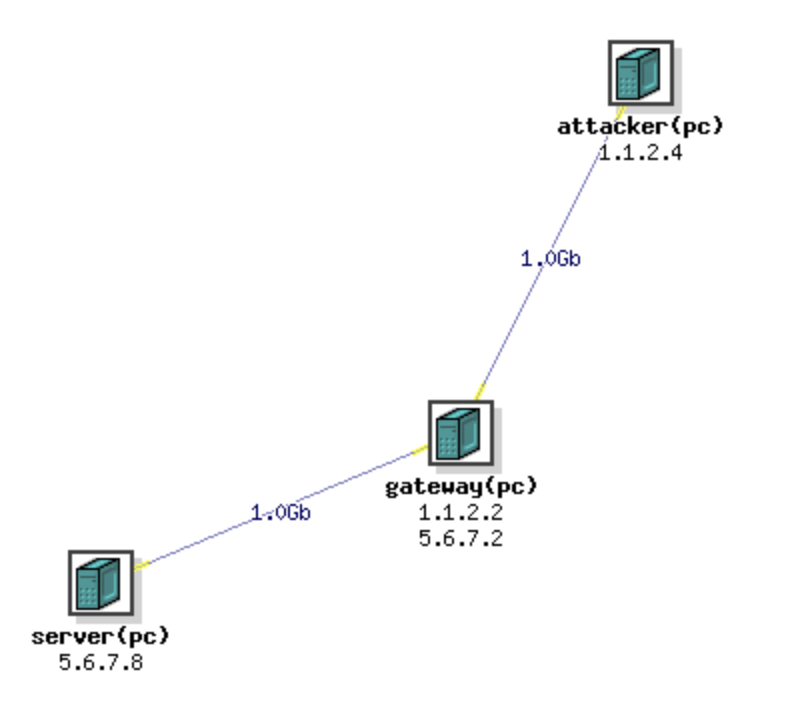
\includegraphics[width=0.44\textwidth]{../drawable/network.png}
  \caption{The network.}
\end{figure}

\subsection{Reconnaisance}

We already know that the range is \verb=5.6.7.0/24=. So we don't have to scan randomly. Our first request is to do an ICMP scan. The bash script is the following:

\begin{code}{Bash script for pinging all hosts.}
  #!/bin/bash
  
  i=1
  end=254

  while [ $i -le $end ]; do
    ping -c 3 5.6.7.$i
    i=$(($i+1))
  done
\end{code}

Since it's a \verb=/24= subnet we can just iterate from 1 to 254 (we skip 0 and 255 for the usual network reasons). Either way, nobody answered to our pings - probably the hosts have disabled ICMP on their end.

With nmap, we can blast our way through with \verb=sudo nmap -sn -PE 5.6.7.0/24=. Still, nobody cared about our pings.

We then tried to do a TCP ACK ping: \verb=sudo nmap -sn -PA 5.6.7.0/24=. This type of ping sends an empty TCP packet with the ACK flag to port 80 (by default, but it's changeable). This usually allows to ignore firewalls. This time, \verb=5.6.7.8= answered!

\begin{figure}[h!]
  \centering
  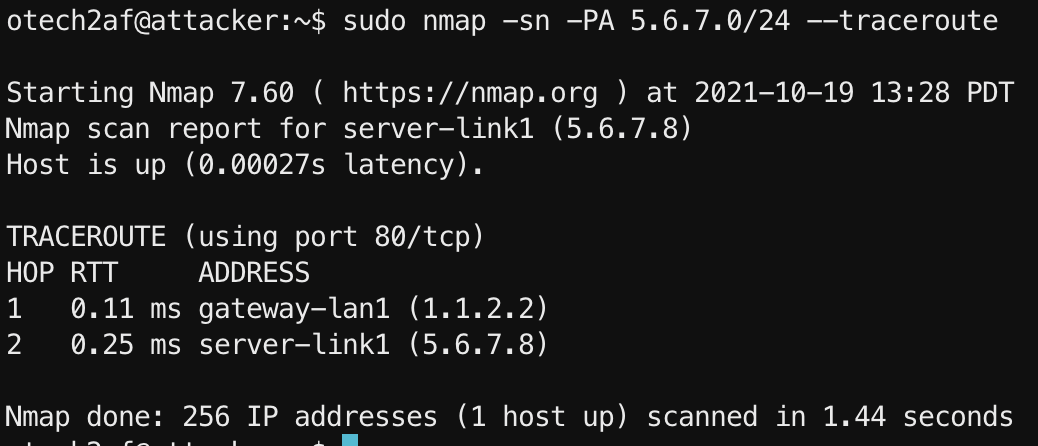
\includegraphics[width=0.66\textwidth]{../drawable/discovery-ack-ping.png}
  \caption{Executing a TCP ACK ping.}
\end{figure}

Finally, we had to probe the network with different probes. A quick visit to the nmap manual yields some useful information:

\begin{itemize}
  \item PS/PA/PU/PY[portlist]: TCP SYN/ACK, UDP or SCTP discovery to given ports
  \item PE/PP/PM: ICMP echo, timestamp, and netmask request discovery probes
  \item PO[protocol list]: IP Protocol Ping
\end{itemize}

To get started, we launched a multi-probe scan: \verb=sudo nmap -sn 5.6.7.0/24=. This does an ICMP echo request, a TCP SYN packet to port 443, a TCP ACK packet to port 80, and an ICMP timestamp request. The result do remain still the same, though. In other cases, such scans can be very useful in order to trick firewalls or avoid protections. For exampke, ICMP PP and PM scans are very useful if PE is blocked - for example, if the server blocked ICMP ping responses.

\subsection{Port scanning}

Our first request is to perform a TCP half open scan. We can do it with \verb|sudo nmap -sS 5.6.7.8|. 

First, we launch it with no flags, then we set the port flag to \verb|-p 1-1500|, in order to scan the first 1500 ports. When no flag is set, nmap defaults to searching on the top 1000 ports - where top refers to the most used, using a nmap-specific metric obtained with experimental results. 

So, we launch another scan with \verb|sudo nmap -sS -p 1-1500 5.6.7.8|.

\begin{figure}[h!]
  \centering
  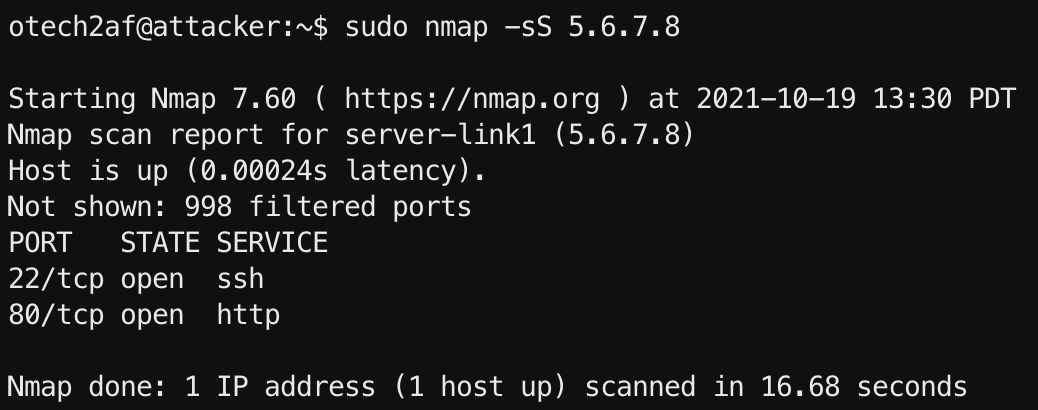
\includegraphics[width=0.66\textwidth]{../drawable/enumeration-stealth-top.png}
  \caption{Executing a TCP half open scan with no flags.}
\end{figure}

\begin{figure}[h!]
  \centering
  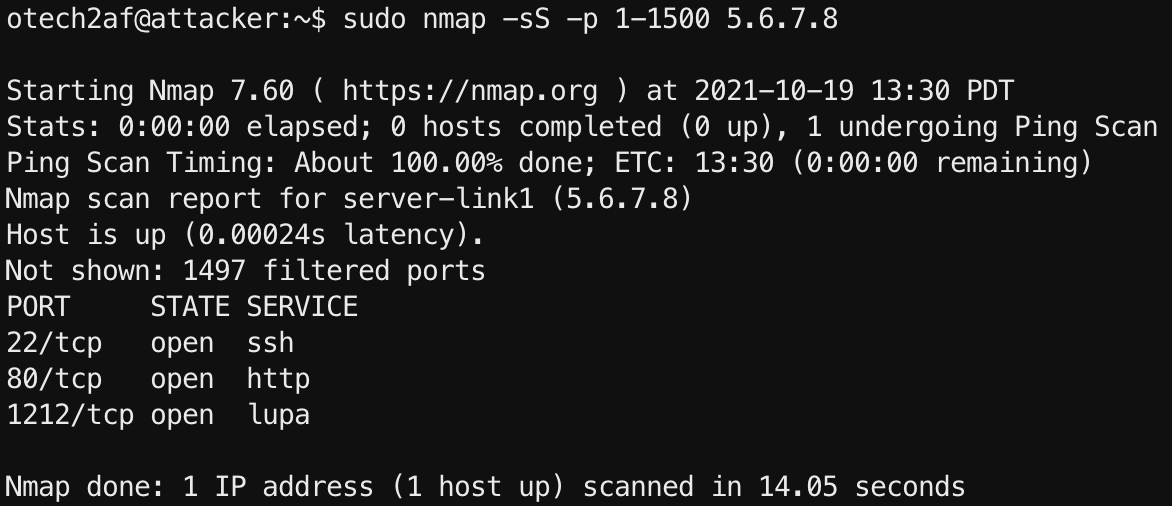
\includegraphics[width=0.66\textwidth]{../drawable/enumeration-stealth-first1500.png}
  \caption{Executing a TCP half open scan with the first 1500 ports.}
\end{figure}

The difference is evident: on our second scan, there is port 1212/tcp open, which is apparently not on the top 1000 ports (being quite an obscure one actually). Indeed, doing:

\begin{verbatim}
  sort -r -k3 /usr/share/nmap/nmap-services | head -n 1000 | grep " 1212"
\end{verbatim}

confirms our suspects.

Next on the list, is performing a XMas scan. It sets the FIN, PSH, and URG flags, lighting the packet up like a Christmas tree. We gest started by launching \verb=sudo nmap -sX 5.6.7.8=.

\begin{figure}[h!]
  \centering
  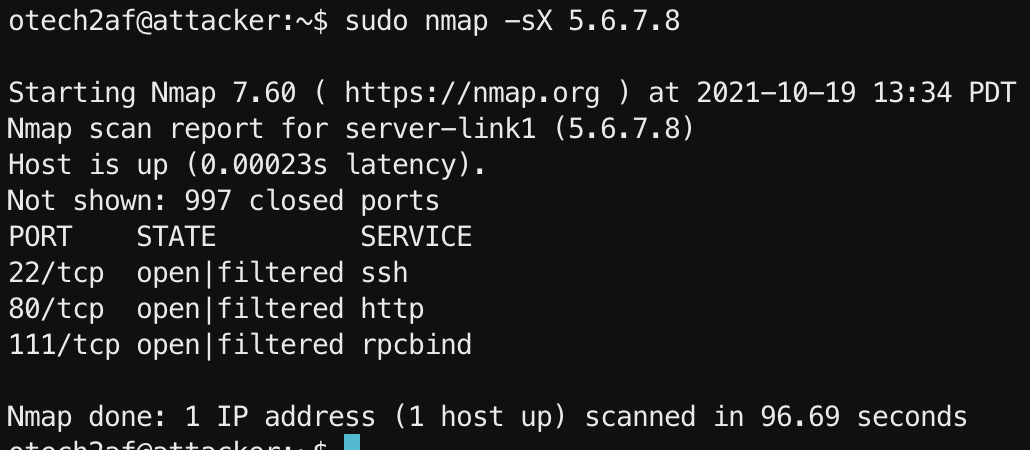
\includegraphics[width=0.66\textwidth]{../drawable/enumeration-xmas.png}
  \caption{Executing a XMas scan.}
\end{figure}

From the results, it looks like we found another \verb=open|filtered= one, rpcbind @ 111/filtered. But why are ports being shown as \verb=open|filtered=?.

As a clarification, from the standpoint of this scan, if a RST packet is received, the port is considered closed. The port is marked surely filtered if we receive an ICMP error. Finally, no response means it is open|filtered.

But now, we have no way of distinguishing a filtered port from an open one - we finished our possible cases - and since open ports are inferred via no responses being generated, we have no way of actually distinguishing them and we have to do additional scans to confirm our findings.

Now, we are required to perform a TCP ACK scan. We can do it with \verb=sudo nmap -sA 5.6.7.8=.

\begin{figure}[h!]
  \centering
  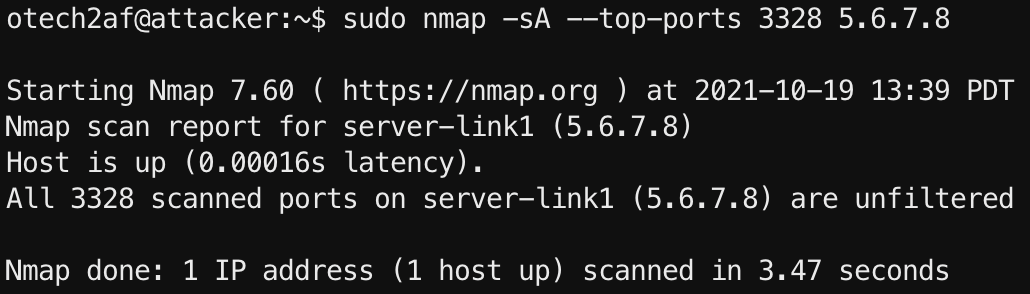
\includegraphics[width=0.66\textwidth]{../drawable/enumeration-ack.png}
  \caption{Executing a TCP ACK scan.}
\end{figure}

All ports seem to be unfiltered - indeed, this is the use of this type of scan: verifying the capabilities of the firewall. This allows us to assume that the firewall is stateless (since the ACKs did correctly go through).

\subsection{OS detection}

Finally, we run a scan to determine both the O.S. version running on the host and the versions of the
services:

\begin{verbatim}
sudo nmap -A -O -sV -sC --traceroute 5.6.7.8  
\end{verbatim}

\begin{figure}[h!]
  \centering
  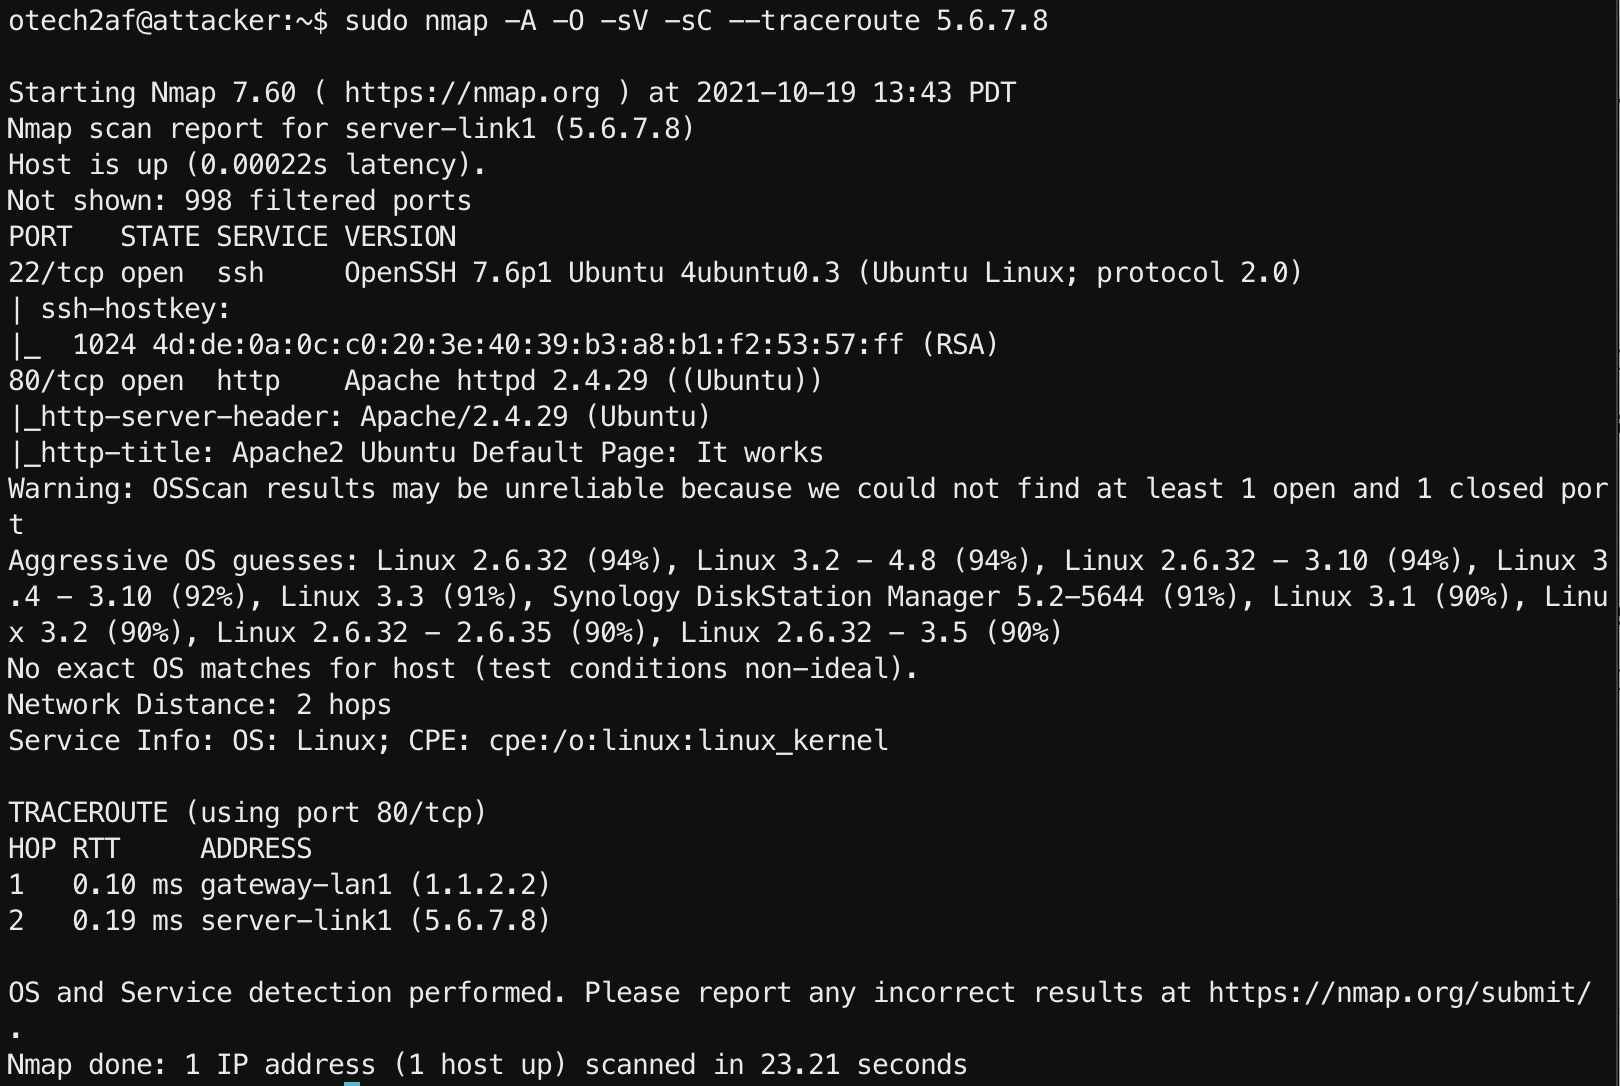
\includegraphics[width=0.8\textwidth]{../drawable/os-versions.png}
  \caption{Executing the final OS discovery scan.}
\end{figure}

From this large message we can gather a lot of information. First, we learn the versions of SSH and Apache (quite an old one). Then, we learn almost surely that our target is running some version of Ubuntu, although the Nmap guesses are wild (the server is actually running Ubuntu 18.04, which is quite newer than the predicted Linux 2.6.32 kernel, whose release dates back to 2012). 

Finally, we learn that our path to the target goes through an additional machine, called \verb=gateway=.
\endgroup
\end{document}